\pagebreak
\section{Chapter by Bartosz Grzybowski}
\label{sec:bartek}
Tutaj mamy zdjecie całkiem niezłej kaczki w naturalnym środowisku kaczek:

\begin{figure}[htbp]
\centering
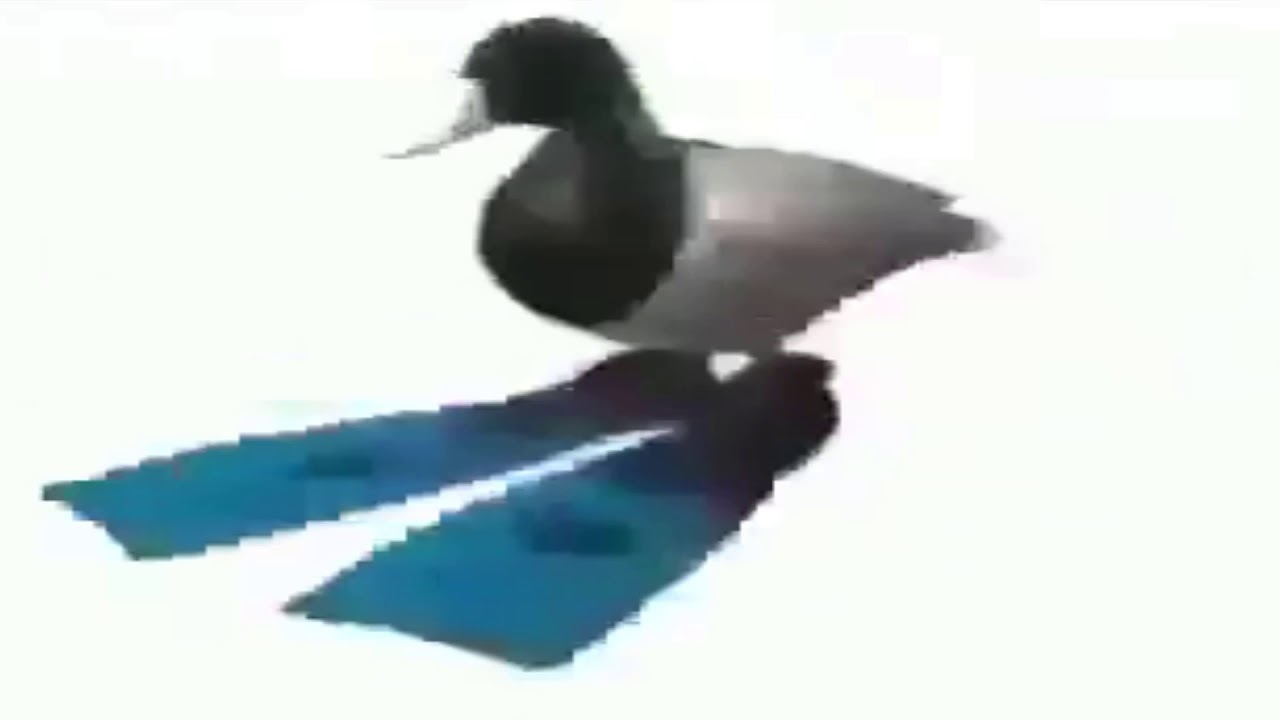
\includegraphics[width=1.0\textwidth]{Pictures/duck.jpg}
\caption{Kaczki dzieki płetwom pływaja znacznie szybciej}
\label{fig:duck}
\end{figure}
\bigskip
Tabela~\ref{tab:tabela_bg} przedstawiajaca tygodniowy plan zajec
\begin{table}[htbp]
\begin{tabular}{|l|ccccc|}
\hline
Lp &
  \multicolumn{1}{l|}{poniedziałek} &
  \multicolumn{1}{l|}{wtorek} &
  \multicolumn{1}{l|}{środa} &
  \multicolumn{1}{l|}{czwartek} &
  \multicolumn{1}{l|}{piatek} \\ \hline
1 & \multicolumn{1}{c|}{wyspać sie} & \multicolumn{1}{c|}{wyspać sie} & \multicolumn{1}{c|}{wyspać sie} & \multicolumn{1}{c|}{postarać sie wyspać} & nawet nie próbować \\ \hline
2 &
  \multicolumn{5}{c|}{zastanowić sie, dlaczego nie jestem wyspany} \\ \hline
3 &
  \multicolumn{5}{c|}{wypić dużo kawy} \\ \hline
4 &
  \multicolumn{1}{c|}{robić matematyke} &
  \multicolumn{1}{c|}{tu też} &
  \multicolumn{1}{c|}{tu też ale mniej} &
  \multicolumn{1}{c|}{niedługo weekend} &
  to już \\ \hline
\end{tabular}
\label{tab:tabela_bg}
\caption{Mozemy tu zauwazyć typowe problemy}
\end{table}
\newpage

Tutaj mamy przykładowe wyrażenie, którego nie umiem policzyć (ale naucze sie jak to zrobić): 

\begin{math}
\lim_{n \to 0} [\frac{(x^2+1-x^2)^4-1}{x}] = ?
\end{math}

Lista z kropkami:

\begin{itemize}
  \item jeden
  \item dwa
  \item trzy
  \item cztery
\end{itemize}

Lista numerowana

\begin{enumerate}
  \item pierwszy
  \item środkowy
  \item też środkowy
  \item ostatni
\end{enumerate}

\bigskip


\textbf{Kofeina}– organiczny zwiazek chemiczny, alkaloid purynowy znajdujacy sie w \underline{ziarnach kawy} i wielu innych surowcach roślinnych. Może również być otrzymywana syntetycznie. Została odkryta przez niemieckiego chemika Friedricha Ferdinanda Rungego w 1819 roku.